\pagebreak
\section{Results and Discussion}
\label{sec:results}

In this section we provide some of the most relevant results we got during the development phase.
We are considering five principal milestones that, within many different trials, led us to improve significantly our MAP score and the overall number of relevant documents actually retrieved.


    \begin{table}[h]
    \centering
    \begin{tabular}{ |l|c|c|c|c|c| }
        \hline
        metric & run1 & run2  & run3 & run4 &run 5 \\ \hline
        num\_q & 663 & 663 & 669 & 669 & 667 \\ \hline
        num\_ret & 654909 & 655684 & 658446 & 658347 & 657903 \\ \hline
        num\_rel & 2571 & 2571 & 2611 & 2611 & 2600 \\ \hline
        num\_rel\_ret & 1914 & 2084 & 2182 & 2191 & 2232 \\ \hline
        map & 0.1553 & 0.1875 & 0.2022 & 0.2029 & 0.2351 \\ \hline
        gm\_map & 0.0178 & 0.0348 & 0.046 & 0.0459 & 0.0629 \\ \hline
        Rprec & 0.1276 & 0.1571 & 0.1697 & 0.1628 & 0.2022 \\ \hline
        bpref & 0.3331 & 0.3626 & 0.3734 & 0.3761 & 0.3861 \\ \hline
        recip\_rank & 0.261 & 0.3037 & 0.3287 & 0.3281 & 0.3945 \\ \hline
        iprec\_at\_recall\_0.00 & 0.2775 & 0.3242 & 0.3499 & 0.3526 & 0.4182 \\ \hline
        iprec\_at\_recall\_0.10 & 0.2771 & 0.3236 & 0.3494 & 0.3523 & 0.4175 \\ \hline
        iprec\_at\_recall\_0.20 & 0.2577 & 0.3076 & 0.3324 & 0.337 & 0.3927 \\ \hline
        iprec\_at\_recall\_0.30 & 0.2113 & 0.2523 & 0.2679 & 0.2743 & 0.3236 \\ \hline
        iprec\_at\_recall\_0.40 & 0.1732 & 0.2152 & 0.2316 & 0.2323 & 0.2716 \\ \hline
        iprec\_at\_recall\_0.50 & 0.1614 & 0.2036 & 0.2193 & 0.2192 & 0.2533 \\ \hline
        iprec\_at\_recall\_0.60 & 0.133 & 0.1636 & 0.1786 & 0.1758 & 0.2014 \\ \hline
        iprec\_at\_recall\_0.70 & 0.1061 & 0.1281 & 0.1402 & 0.1402 & 0.1552 \\ \hline
        iprec\_at\_recall\_0.80 & 0.0892 & 0.1091 & 0.1178 & 0.12 & 0.1295 \\ \hline
        iprec\_at\_recall\_0.90 & 0.0742 & 0.0896 & 0.0956 & 0.0992 & 0.1033 \\ \hline
        iprec\_at\_recall\_1.00 & 0.0741 & 0.0895 & 0.0954 & 0.0986 & 0.1028 \\ \hline
        P\_5 & 0.1222 & 0.1475 & 0.1599 & 0.1614 & 0.1874 \\ \hline
        P\_10 & 0.0973 & 0.1192 & 0.1296 & 0.1312 & 0.1432 \\ \hline
        P\_15 & 0.0797 & 0.0965 & 0.1049 & 0.1068 & 0.1135 \\ \hline
        P\_20 & 0.0668 & 0.0805 & 0.088 & 0.0891 & 0.0935 \\ \hline
        P\_30 & 0.0519 & 0.0616 & 0.0661 & 0.0668 & 0.0703 \\ \hline
        P\_100 & 0.0206 & 0.0236 & 0.0256 & 0.0258 & 0.0268 \\ \hline
        P\_200 & 0.0116 & 0.0132 & 0.014 & 0.0141 & 0.0148 \\ \hline
        P\_500 & 0.0053 & 0.0059 & 0.0061 & 0.0061 & 0.0064 \\ \hline
        P\_1000 & 0.0029 & 0.0031 & 0.0033 & 0.0033 & 0.0033 \\ \hline
    \end{tabular}

\end{table}


\begin{figure}[h!]
    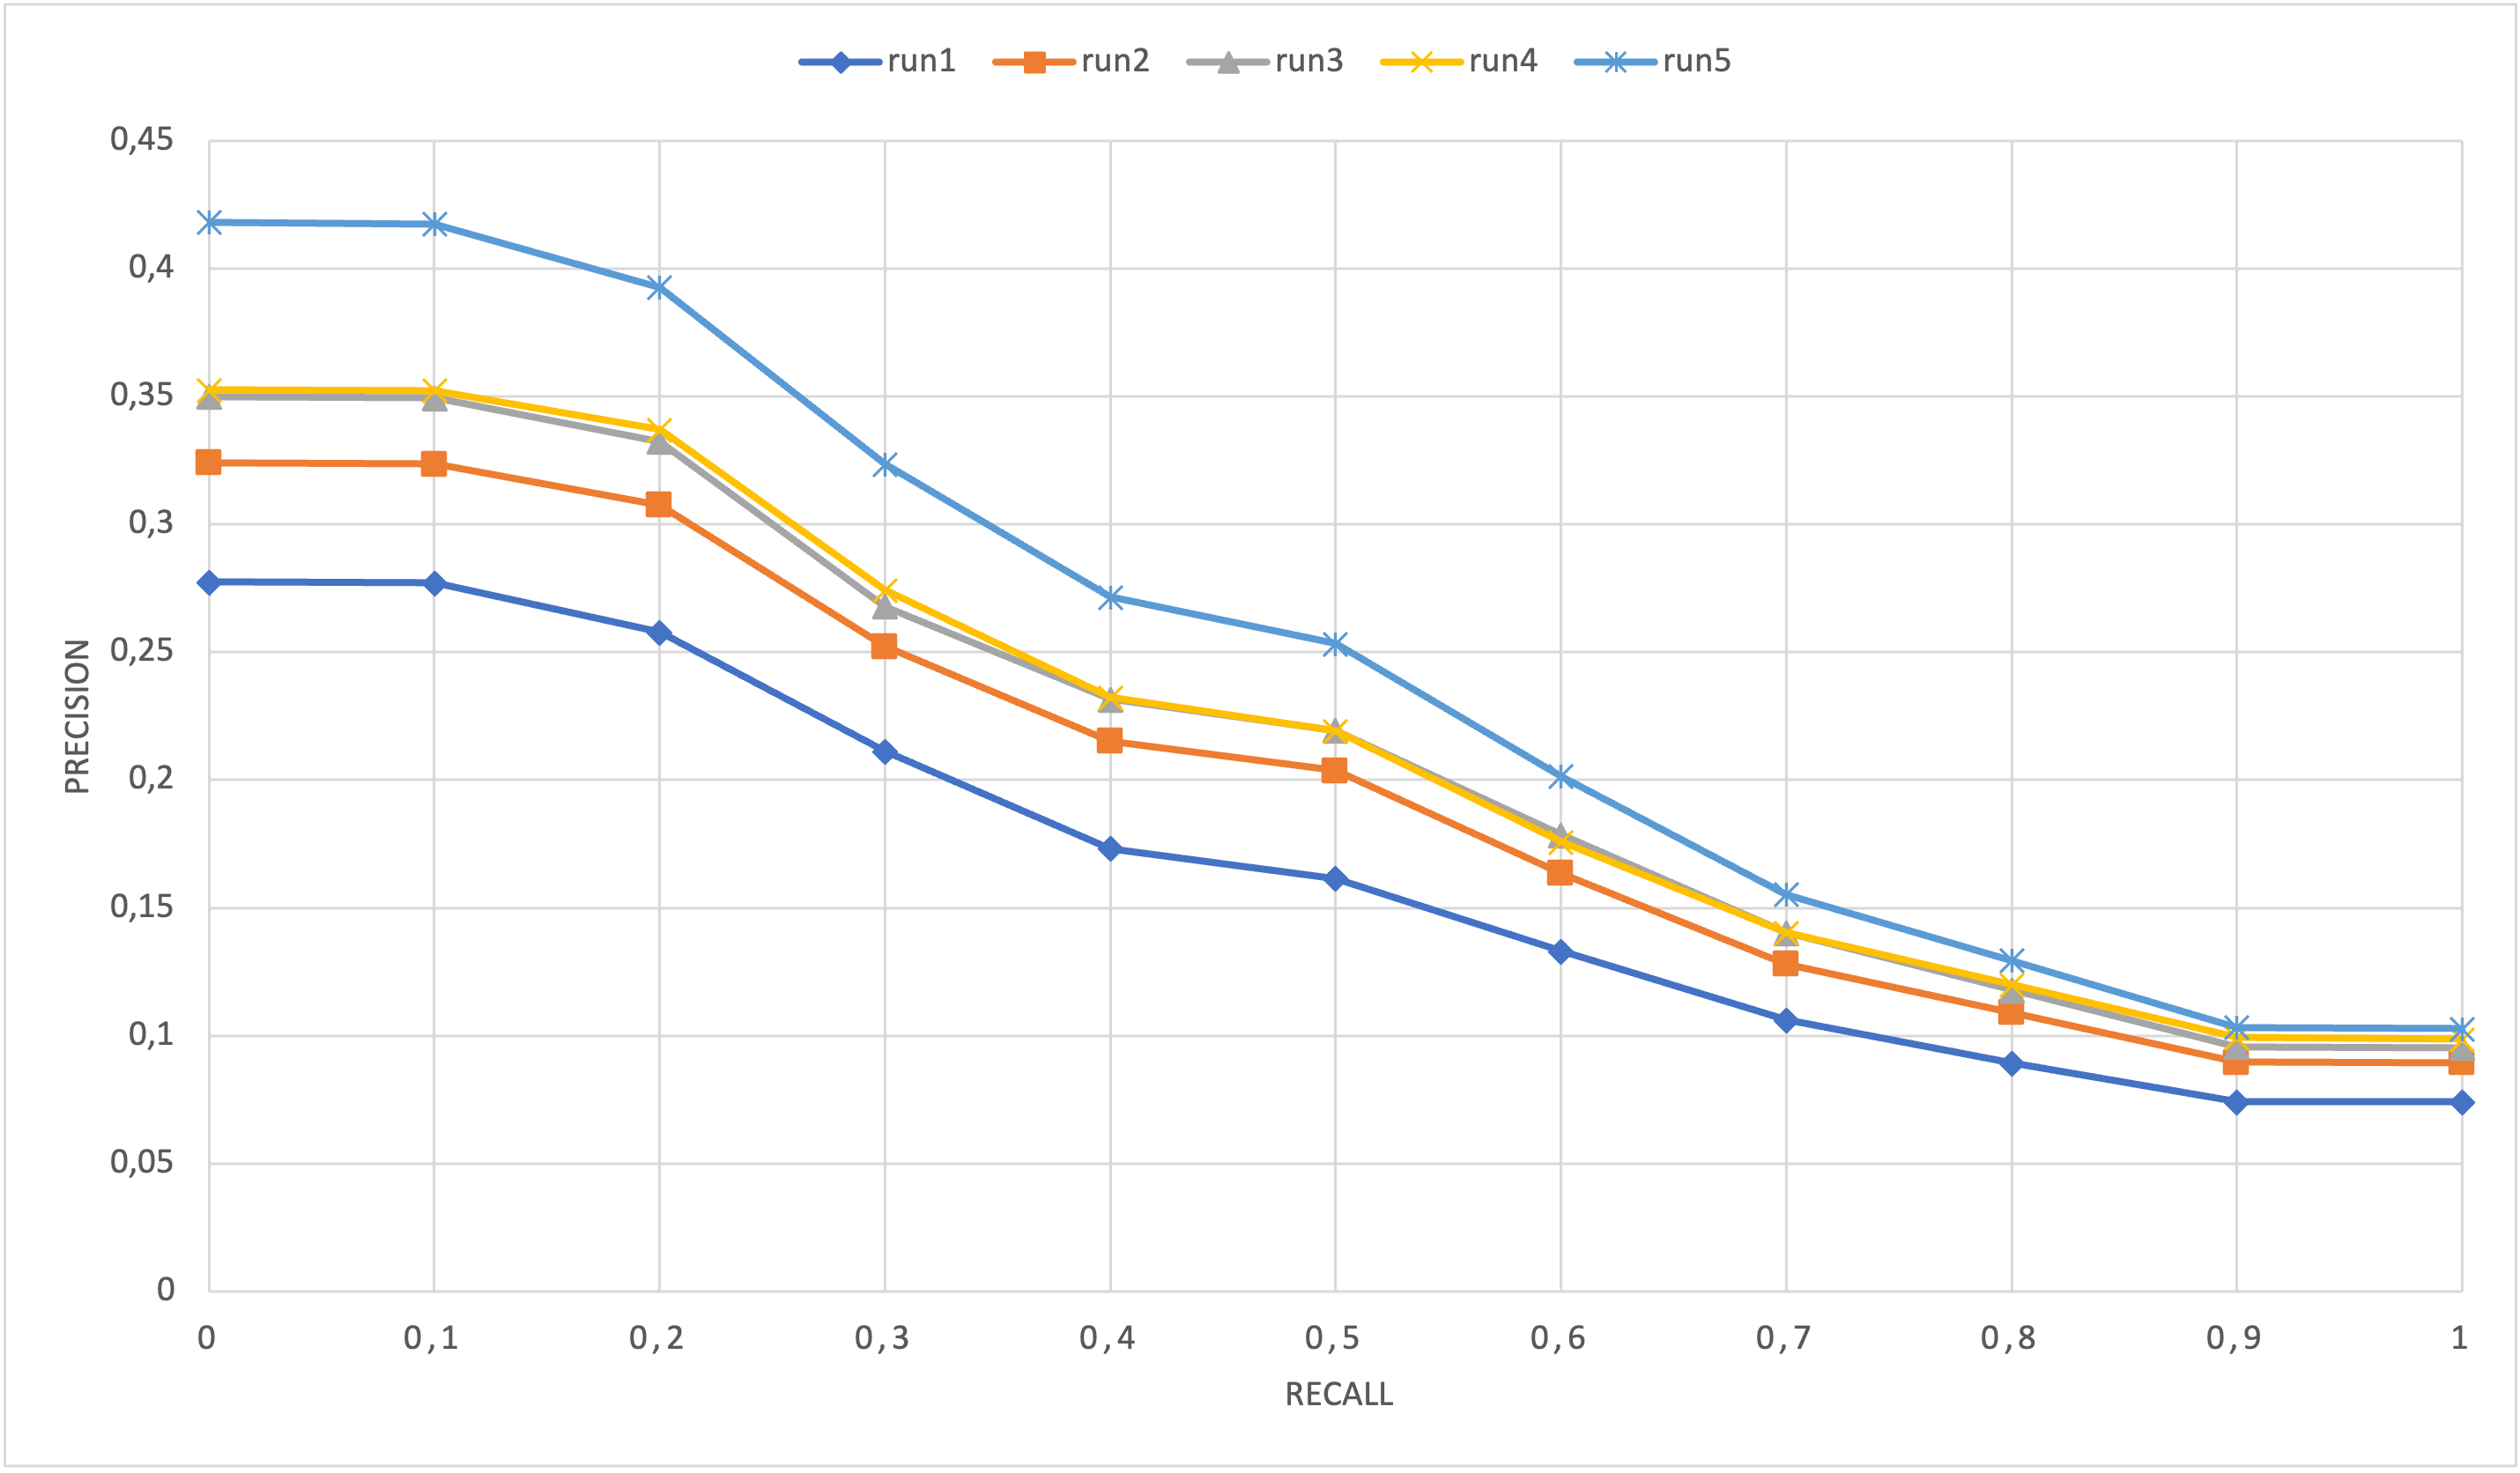
\includegraphics[width=\textwidth]{figure/rp_french.png}
    \caption{Recall and precision graph}
    \label{fig:rp_french}
\end{figure}

First of all, given that we were provided with two different version of the same document's \textit{corpora}, our first idea was to try with english version.\\ 
We noticed that the best combination of basic IR tools were to use the Porter stemmer, a lenght filter from 1 to 10, and a list of stopword composed by some standard terms and more from the top 600 extracted from the index.
The very first big milestone, that helped us to increment the MAP of around 3.5 points, was the JavaScript code cleaer, since we noticed by inspection that many documents were having JS scripts inside.\\
Always by inspecting some documents and queries, and also considering that the original collection was the french version (translated then in english), we observed that the translation was very poor: by switching to french
with just cleaning the JS code and some other minor cleaning tools, without even using an adequate stoplist and a correct stemmer for the french language, the MAP was increasing by 5 percentual points; 2 more points were achieved with
a stop list built for french in the same way we did for previously for english, the \textit{FrenchLightStemFilter} as stemmer, and moving the lenght filter from 2 to 15 (as french probabily usually has longer words).
We tried some NLP techniques for english, in particular using \textit{Part-Of-Speech} techniques, to see if there were improvements, and in case apply it to our main implementation for french with an appropriate model, but results 
were not interesting, and also the computing time were definitely too costly.
Another approach we tried and that carried an improvement was to use \textit{Query expansion}: we used some generative text models to expand our queries: we then decided to weight different query scores by boosting the original one linearly with respect to the number
of expansion used, and without boosting the expansion: this carried to us an extra MAP point.
We tried to combine different similarities rather than using the classic BM25Similarity: we tried to use the Lucene MultiSimilarity, that allows to combine equally the score of two or more similarity scores, but it does not allow to
tune the weights. Then, we tried to reimplement the MultiSimilarity class with tuning options, but results were always lower than the standard BM25Similarity. Some minor improvements came up by fine tuning the document-length
normalization \textit{b} parameter and the term frequency component \textit{k1} parameter of the BM25Similarity.
The last main implementation we did was to use some \textit{Reranking} techniques:  
Lastly, some minor addings were setted on the analyzer by implementing the Lucene ElisionFilter (for french), that aims to remove apostrophed articles and prepositions from tokens (for example, \textit{m'appelle} and \textit{t'appelle} become the same token).


